% Options for packages loaded elsewhere
\PassOptionsToPackage{unicode}{hyperref}
\PassOptionsToPackage{hyphens}{url}
\PassOptionsToPackage{dvipsnames,svgnames,x11names}{xcolor}
%
\documentclass[
  a4paper]{article}

\usepackage{amsmath,amssymb}
\usepackage{iftex}
\ifPDFTeX
  \usepackage[T1]{fontenc}
  \usepackage[utf8]{inputenc}
  \usepackage{textcomp} % provide euro and other symbols
\else % if luatex or xetex
  \usepackage{unicode-math}
  \defaultfontfeatures{Scale=MatchLowercase}
  \defaultfontfeatures[\rmfamily]{Ligatures=TeX,Scale=1}
\fi
\usepackage{lmodern}
\ifPDFTeX\else  
    % xetex/luatex font selection
\fi
% Use upquote if available, for straight quotes in verbatim environments
\IfFileExists{upquote.sty}{\usepackage{upquote}}{}
\IfFileExists{microtype.sty}{% use microtype if available
  \usepackage[]{microtype}
  \UseMicrotypeSet[protrusion]{basicmath} % disable protrusion for tt fonts
}{}
\makeatletter
\@ifundefined{KOMAClassName}{% if non-KOMA class
  \IfFileExists{parskip.sty}{%
    \usepackage{parskip}
  }{% else
    \setlength{\parindent}{0pt}
    \setlength{\parskip}{6pt plus 2pt minus 1pt}}
}{% if KOMA class
  \KOMAoptions{parskip=half}}
\makeatother
\usepackage{xcolor}
\setlength{\emergencystretch}{3em} % prevent overfull lines
\setcounter{secnumdepth}{5}
% Make \paragraph and \subparagraph free-standing
\makeatletter
\ifx\paragraph\undefined\else
  \let\oldparagraph\paragraph
  \renewcommand{\paragraph}{
    \@ifstar
      \xxxParagraphStar
      \xxxParagraphNoStar
  }
  \newcommand{\xxxParagraphStar}[1]{\oldparagraph*{#1}\mbox{}}
  \newcommand{\xxxParagraphNoStar}[1]{\oldparagraph{#1}\mbox{}}
\fi
\ifx\subparagraph\undefined\else
  \let\oldsubparagraph\subparagraph
  \renewcommand{\subparagraph}{
    \@ifstar
      \xxxSubParagraphStar
      \xxxSubParagraphNoStar
  }
  \newcommand{\xxxSubParagraphStar}[1]{\oldsubparagraph*{#1}\mbox{}}
  \newcommand{\xxxSubParagraphNoStar}[1]{\oldsubparagraph{#1}\mbox{}}
\fi
\makeatother


\providecommand{\tightlist}{%
  \setlength{\itemsep}{0pt}\setlength{\parskip}{0pt}}\usepackage{longtable,booktabs,array}
\usepackage{calc} % for calculating minipage widths
% Correct order of tables after \paragraph or \subparagraph
\usepackage{etoolbox}
\makeatletter
\patchcmd\longtable{\par}{\if@noskipsec\mbox{}\fi\par}{}{}
\makeatother
% Allow footnotes in longtable head/foot
\IfFileExists{footnotehyper.sty}{\usepackage{footnotehyper}}{\usepackage{footnote}}
\makesavenoteenv{longtable}
\usepackage{graphicx}
\makeatletter
\newsavebox\pandoc@box
\newcommand*\pandocbounded[1]{% scales image to fit in text height/width
  \sbox\pandoc@box{#1}%
  \Gscale@div\@tempa{\textheight}{\dimexpr\ht\pandoc@box+\dp\pandoc@box\relax}%
  \Gscale@div\@tempb{\linewidth}{\wd\pandoc@box}%
  \ifdim\@tempb\p@<\@tempa\p@\let\@tempa\@tempb\fi% select the smaller of both
  \ifdim\@tempa\p@<\p@\scalebox{\@tempa}{\usebox\pandoc@box}%
  \else\usebox{\pandoc@box}%
  \fi%
}
% Set default figure placement to htbp
\def\fps@figure{htbp}
\makeatother

\usepackage[catalan]{babel}
\usepackage{fancyhdr}
\pagestyle{fancy}
\fancyhead{}
\fancyhead[C]{Anàlisi de dades òmiques}
\fancyhead[L]{Ricard Gonzalez}
\fancyhead[R]{\today}
\usepackage{booktabs}
\usepackage{longtable}
\usepackage{array}
\usepackage{multirow}
\usepackage{wrapfig}
\usepackage{float}
\usepackage{colortbl}
\usepackage{pdflscape}
\usepackage{tabu}
\usepackage{threeparttable}
\usepackage{threeparttablex}
\usepackage[normalem]{ulem}
\usepackage{makecell}
\usepackage{xcolor}
\makeatletter
\@ifpackageloaded{caption}{}{\usepackage{caption}}
\AtBeginDocument{%
\ifdefined\contentsname
  \renewcommand*\contentsname{Table of contents}
\else
  \newcommand\contentsname{Table of contents}
\fi
\ifdefined\listfigurename
  \renewcommand*\listfigurename{List of Figures}
\else
  \newcommand\listfigurename{List of Figures}
\fi
\ifdefined\listtablename
  \renewcommand*\listtablename{List of Tables}
\else
  \newcommand\listtablename{List of Tables}
\fi
\ifdefined\figurename
  \renewcommand*\figurename{Figure}
\else
  \newcommand\figurename{Figure}
\fi
\ifdefined\tablename
  \renewcommand*\tablename{Table}
\else
  \newcommand\tablename{Table}
\fi
}
\@ifpackageloaded{float}{}{\usepackage{float}}
\floatstyle{ruled}
\@ifundefined{c@chapter}{\newfloat{codelisting}{h}{lop}}{\newfloat{codelisting}{h}{lop}[chapter]}
\floatname{codelisting}{Listing}
\newcommand*\listoflistings{\listof{codelisting}{List of Listings}}
\makeatother
\makeatletter
\makeatother
\makeatletter
\@ifpackageloaded{caption}{}{\usepackage{caption}}
\@ifpackageloaded{subcaption}{}{\usepackage{subcaption}}
\makeatother

\usepackage{bookmark}

\IfFileExists{xurl.sty}{\usepackage{xurl}}{} % add URL line breaks if available
\urlstyle{same} % disable monospaced font for URLs
\hypersetup{
  pdftitle={PAC1 - Anàlisi de dades òmiques},
  pdfauthor={Ricard Gonzalez},
  colorlinks=true,
  linkcolor={blue},
  filecolor={Maroon},
  citecolor={Blue},
  urlcolor={Blue},
  pdfcreator={LaTeX via pandoc}}


\title{PAC1 - Anàlisi de dades òmiques}
\author{Ricard Gonzalez}
\date{2025-03-29}

\begin{document}
\maketitle

\renewcommand*\contentsname{Índex}
{
\hypersetup{linkcolor=}
\setcounter{tocdepth}{3}
\tableofcontents
}

\newpage

\section{Resum}\label{resum}

\section{Objectius}\label{objectius}

Aquest informe està dedicat al compliment d'una sèrie d'objectius,
esmentats a continuació:

\begin{enumerate}
\def\labelenumi{\arabic{enumi}.}
\item
  Seleccionar un conjunt de dades (``\emph{dataset}'') de metabolòmica
  per al seu ús durant l'informe.
\item
  Construïr, a partir d'aquest \emph{dataset}, un objecte de tipus
  \emph{SummarizedExperiment}.
\item
  Comparar, a nivell conceptual, l'objecte de tipus
  \emph{SummarizedExperiment} amb el seu predecessor
  \emph{ExpressionSet}.
\item
  Dur a terme una anàlisi exploratòria de les dades.
\item
  Organitzar la informació, mètodes emprats, resultats de l'anàlisi i
  discussió i conclusions sobre aquests en un informe estructurat.
\item
  Creació d'un repositori de GitHub, esmentat al propi informe, on s'hi
  recullin totes les dades i materials necessaris per a replicar
  l'anàlisi descrit a l'informe.
\end{enumerate}

Alguns dels objectius tindràn cabuda explícita a l'informe (per exemple,
l'anàlisi exploratòria de les dades). Altres, en canvi (com la creació
del propi informe, o la generació d'un repositori de GitHub) son
purament operatius i per tant se'n presentaràn els entregables
directament (el propi informe, o un enllaç d'accés al repositori,
respectivament).

\pagebreak

\section{Mètodes}\label{muxe8todes}

\subsection{Tria del conjunt de dades}\label{tria-del-conjunt-de-dades}

Per aquest informe, es van considerar diversos conjunts de dades
metabolòmiques presents al repositori proveït per l'assignatura.

Entre d'altres, hi havia conjunts de dades sobre estudis de cancer
gàstric, assajos de fosfoproteòmica o pèrdua de massa muscular
(caquèxia).

El conjunt de dades escollit ha estat el ``2024-Cachexia'', obtingut del
repositori en format valors separats per comes (.CSV, per les seves
sigles en anglès). Al llarg de l'informe, s'anomenarà \emph{cachexia}
per facilitar la lectura.

Els motius que justifiquen la tria d'aquest conjunt de dades han estat
el seu bon balanç cardinalitat/dimensionalitat (més mostres que
dimensions), el fet que totes les variables no-metadades eren
numèriques, i la claredat del conjunt de dades (sense valors perduts).

Altres conjunts de dades, tot i interessants, tenien especificitats que
els feien poc pràctics per un exercici centrat en entendre aspectes
bàsics de Bioconductor, la programació orientada a objectes i la
familiarització bàsica amb dades òmiques.

Aquest conjunt de dades recull anàlisis d'orina de 77 pacients, 47 dels
quals presenten caquèxia i els 30 restants son controls. De cada mostra,
s'hi han determinat experimentalment els valors de 63 metabòlits.

\subsection{Paquets de software
utilitzats}\label{paquets-de-software-utilitzats}

Per a la interacció amb les dades, es va utilitzar la versió
\emph{4.4.2} de \textbf{R}, i la versió de \textbf{RStudio}
\emph{2024.12.1+563}. L'informe es va generar mitjançant el paquet
\textbf{quarto} en la seva versió \emph{1.4.4}.

Es van importar les dades mitjançant el paquet \textbf{data.table}, en
la seva versió \emph{1.17.0}.

Respecte la manipulació de les dades, es va fer servir
\textbf{Bioconductor} en la seva versió \emph{3.20}, del què es van
utilitzar els paquets \textbf{Biobase} en la versió \emph{2.66.0} i
\textbf{SummarizedExperiment} en la versió \emph{1.36.0}. També es van
utilitzar funcions del paquet \textbf{S4Vectors}, en la versió
\emph{0.44.0}.

Per a l'anàlisi de les dades només es van utilitzar funcions del paquet
\textbf{stats}, inclòs amb R. Per tant, no és requisit configurar
versions addicionals de paquets per a l'anàlisi més enllà de la versió
de R.

Finalment, la presentació i visualització de les dades en figures i
taules es va fer amb els paquets \textbf{ggplot2}, en versió
\emph{3.5.1}, \textbf{kableExtra}, en versió \emph{1.4.0} i
\textbf{showtext}, en versió \emph{0.9-7}.

\subsection{Creació de l'objecte
SummarizedExperiment}\label{creaciuxf3-de-lobjecte-summarizedexperiment}

Per a la generació d'un objecte de tipus \emph{SummarizedExperiment} a
partir del conjunt de dades \emph{cachexia}, es va seguir una estratègia
metòdica, centrada en la identificació i organització progressiva del
contingut del conjunt de dades per a estructurar-lo en parts de format
desitjat.

En primer lloc, es van separar les metadades (presents a les dues
primeres columnes del conjunt, corresponent a l'identificador únic del
pacient, ``Patient ID'', i al Grup experimental ``Muscle loss'').

Les dades restants es van transformar en matriu transposada: aquest pas
és clau, atès que els objectes \emph{SummarizedExperiment} requereixen
les variables com a files, i les observacions com a columnes. Per
assegurar la integritat de les dades i la consistència relacional, es va
asignar identificadors de pacient tant a la matriu de resultats
metabolòmics com a la taula de metadades.

Es va construïr un objecte \emph{SummarizedExperiment} assignant la
matriu transposada i etiquetada a l'\emph{slot} ``\emph{assays}'', amb
el nom de ``\emph{counts}''. A l'\emph{slot} ``\emph{colData}'' s'hi van
assignar les metadades.

L'objecte es va desar en format binari (.Rda) per facilitar-ne la
reutilització.

\pagebreak

\subsection{Anàlisi exploratori de les
dades}\label{anuxe0lisi-exploratori-de-les-dades}

\subsubsection{Objectius i preparació de les
dades}\label{objectius-i-preparaciuxf3-de-les-dades}

Per a una exploració preliminar de les dades, es va decidir examinar si
era possible capturar els dos ``Grups de tractament'' (els pacients
caquèxics versus els pacients control) en funció de la seva distància
inter-pacient. De manera similar, també es va intentar capturar la
variabilitat entre mostres (i, si fos possible, Grups de tractament) en
funció de la covariància.

Per a resoldre tots dos punts, es va procedir obtenint la matriu de
metabòlits en la seva estructura original (amb els pacients com a files
i els valors de metabòlit com a columnes). Es va etiquetar degudament la
matriu amb codis de pacient i es va normalitzar amb la funció
\emph{scale()}, que per defecte centra i escala les dades a \(\mu = 0\)
i \(\sigma = 1\).

Addicionalment, es va calcular la matriu de distàncies entre pacients a
partir de la matriu normalitzada, mitjançant la mètrica de distància
Euclídia.

\subsubsection{Escalat Multidimensional}\label{escalat-multidimensional}

Per a intentar distingir els pacients a través de la seva distància, es
va utilitzar la matriu de distàncies euclídies per a Escalat
Multidimensional (MDS, per les seves sigles en anglès), mitjançant la
funció \emph{cmdscale()}. Aquesta funció es va utilitzar per obtenir una
representació bidimensional de les dades projectades a través de les
seves distàncies euclídies.

Aquest resultat es va etiquetar posteriorment amb el Grup de tractament
de cada pacient mitjançant el seu identificador, i es van visualitzar
les dades.

\subsubsection{Anàlisi de Components
Principals}\label{anuxe0lisi-de-components-principals}

Finalment, per capturar la variabilitat entre pacients a través de la
seva covariància, es va fer servir un Anàlisi de Components Principals
(PCA).

Amb aquesta finalitat, la matriu normalitzada obtinguda anteriorment es
va sotmetre a descomposició en components principals mitjançant la
funció \emph{prcomp()}. Es va emprar per extreure la projecció de les
dades en cadascuna de les components principals, i les dues primeres
components (PC1 i PC2) es van utilitzar, amb les dades etiquetades, per
visualitzar els pacients en funció del seu Grup de tractament.

\pagebreak

\section{Resultats}\label{resultats}

\subsection{Obtenció de l'objecte
SummarizedExperiment}\label{obtenciuxf3-de-lobjecte-summarizedexperiment}

Seguint la estratègia esmentada als Mètodes, s'ha obtingut un objecte
SummarizedExperiment a partir del conjunt de dades \emph{cachexia}.

\begin{table}
\centering
\caption{Dimensions de l'objecte SummarizedExperiment `dades`.}
\centering
\resizebox{\ifdim\width>\linewidth\linewidth\else\width\fi}{!}{
\fontsize{8}{10}\selectfont
\begin{tabular}[t]{lr}
\toprule
Component & Valor\\
\midrule
\cellcolor{gray!10}{Metabolits} & \cellcolor{gray!10}{63}\\
Mostres & 77\\
\bottomrule
\end{tabular}}
\end{table}

\begin{table}
\centering
\caption{Primeres 5 files i 5 columnes de la matriu de metabolits de l'objecte `dades`.}
\centering
\resizebox{\ifdim\width>\linewidth\linewidth\else\width\fi}{!}{
\fontsize{8}{10}\selectfont
\begin{tabular}[t]{lrrrrr}
\toprule
  & PIF\_178 & PIF\_087 & PIF\_090 & NETL\_005\_V1 & PIF\_115\\
\midrule
\cellcolor{gray!10}{1,6-Anhydro-beta-D-glucose} & \cellcolor{gray!10}{40.85} & \cellcolor{gray!10}{62.18} & \cellcolor{gray!10}{270.43} & \cellcolor{gray!10}{154.47} & \cellcolor{gray!10}{22.20}\\
1-Methylnicotinamide & 65.37 & 340.36 & 64.72 & 52.98 & 73.70\\
\cellcolor{gray!10}{2-Aminobutyrate} & \cellcolor{gray!10}{18.73} & \cellcolor{gray!10}{24.29} & \cellcolor{gray!10}{12.18} & \cellcolor{gray!10}{172.43} & \cellcolor{gray!10}{15.64}\\
2-Hydroxyisobutyrate & 26.05 & 41.68 & 65.37 & 74.44 & 83.93\\
\cellcolor{gray!10}{2-Oxoglutarate} & \cellcolor{gray!10}{71.52} & \cellcolor{gray!10}{67.36} & \cellcolor{gray!10}{23.81} & \cellcolor{gray!10}{1199.91} & \cellcolor{gray!10}{33.12}\\
\bottomrule
\end{tabular}}
\end{table}

\begin{table}
\centering
\caption{Metadades de les primeres 5 mostres de l'objecte `dades`.}
\centering
\resizebox{\ifdim\width>\linewidth\linewidth\else\width\fi}{!}{
\fontsize{8}{10}\selectfont
\begin{tabular}[t]{lll}
\toprule
  & Patient.ID & Muscle.loss\\
\midrule
\cellcolor{gray!10}{PIF\_178} & \cellcolor{gray!10}{PIF\_178} & \cellcolor{gray!10}{cachexic}\\
PIF\_087 & PIF\_087 & cachexic\\
\cellcolor{gray!10}{PIF\_090} & \cellcolor{gray!10}{PIF\_090} & \cellcolor{gray!10}{cachexic}\\
NETL\_005\_V1 & NETL\_005\_V1 & cachexic\\
\cellcolor{gray!10}{PIF\_115} & \cellcolor{gray!10}{PIF\_115} & \cellcolor{gray!10}{cachexic}\\
\bottomrule
\end{tabular}}
\end{table}

\begin{figure}[H]

{\centering \pandocbounded{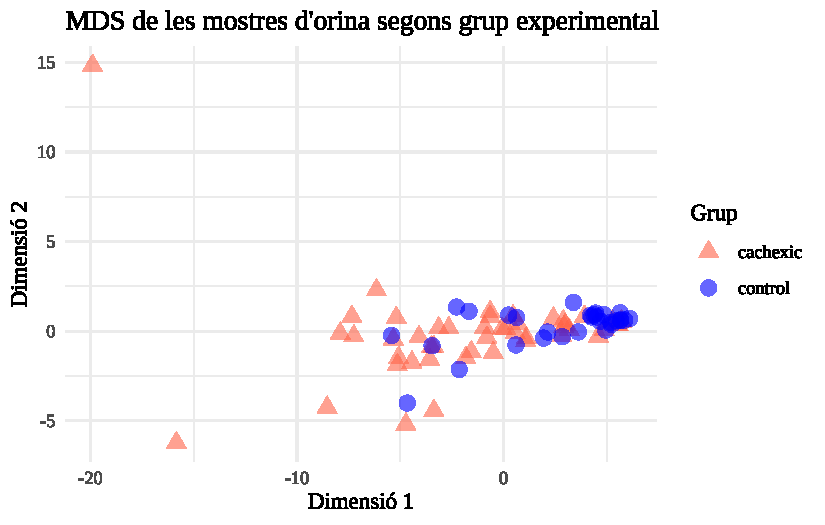
\includegraphics[keepaspectratio]{ricard_gonzalez_PAC1_ADO_files/figure-pdf/unnamed-chunk-6-1.pdf}}

}

\caption{Diagrama de dispersió que mostra la projecció en 2 dimensions
del dataset cachexia transformat via escalat multidimensional (MDS). Els
pacients caquèxics apareixen com a triangles vermells, i els controls
com a cercles blaus.}

\end{figure}%

\begin{figure}[H]

{\centering \pandocbounded{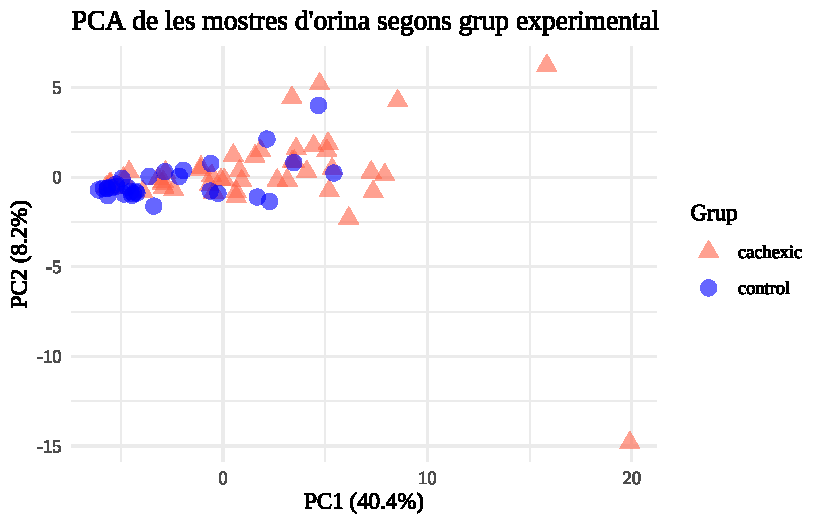
\includegraphics[keepaspectratio]{ricard_gonzalez_PAC1_ADO_files/figure-pdf/unnamed-chunk-7-1.pdf}}

}

\caption{Diagrama de dispersió que mostra la projecció en 2 dimensions
del dataset cachexia transformat via anàlisi de components principals
(PCA). Cada eix inclou entre parèntesi la variància explicada per la
corresponent Component Principal. Els pacients caquèxics apareixen com a
triangles vermells, i els controls com a cercles blaus.}

\end{figure}%

\section{Discussió}\label{discussiuxf3}

\section{Conclusions}\label{conclusions}

\section{Referències}\label{referuxe8ncies}




\end{document}
